\documentclass[usenames,dvipsnames]{beamer}

\usepackage{tikz}
\usepackage{amsmath}
\usepackage{listings}
\usepackage{graphicx}
\usepackage{inconsolata}
\usetheme{LANL}
\usetikzlibrary{positioning}
\usetikzlibrary{shapes.misc}
\graphicspath{{./figs/}}
\usepackage{xcolor}

\lstset{
  basicstyle=\footnotesize\ttfamily,
  breaklines=true,
  moredelim=**[is][\color{BurntOrange}]{@}{@},
  moredelim=**[is][\color{RoyalBlue}]{&}{&},
}
\definecolor{myLightGray}{RGB}{192,192,192}
\setbeamercolor{fakegraphic}{bg=myLightGray,fg=black}

\title{Dominator DAGs}
\subtitle{Generalizing Single Static Assignment}

\author[shortname]{George Stelle}
\institute[shortinst]{Los Alamos National Laboratory}
          
\begin{document}

\begin{frame}
\maketitle
\end{frame}

\begin{frame}
\frametitle{Outline}
\begin{itemize}
\item Single Static Assignment
\item Dominator Trees
\item Dominator DAGs
\item Formalization 
\item Concurrency
\item Questions
\end{itemize}
\end{frame}

\begin{frame}[fragile]
\frametitle{Single Static Assignment (SSA)}
\begin{columns}
\begin{column}{0.35\textwidth}\end{column}
\begin{column}{0.9\textwidth}
\begin{lstlisting}
define f(x){
  entry:
    cond = and x, 1
    br cond, a, b
  a: 
    y = mul 4, x
    call g()
    br cond, b, c 
  b:
    z = add x, x
    call h()
    br cond, c, a
  c: 
    r = add y, z
    ret r
}
\end{lstlisting}
\end{column}
\end{columns}
\end{frame}

\begin{frame}[fragile]
\frametitle{Control Flow Graph (CFG)}
\begin{columns}
\begin{column}{0.1\textwidth}
\end{column}
\begin{column}{0.4\textwidth}
\begin{lstlisting}
define f(x){
  entry:
    cond = and x, 1
    br cond, a, b
  a: 
    y = mul 4, x
    call g()
    br cond, b, c 
  b:
    z = add x, x
    call h()
    br cond, c, a
  c: 
    r = add y, z
    ret r
}
\end{lstlisting}
\end{column}
\begin{column}{0.5\textwidth}
\center
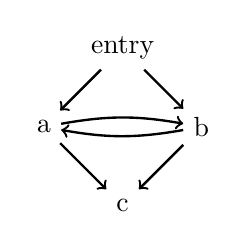
\begin{tikzpicture}[->, line width=0.3mm]
\node(entry) at (2,3) {entry};
\node(a) at (1,2) {a};
\node(b) at (3,2) {b};
\node(c) at (2,1) {c};
\path
  (entry) edge (a)
  (entry) edge (b)
  (a) edge [bend left=10] (b)
  (b) edge [bend left=10] (a)
  (a) edge (c)
  (b) edge (c);
\end{tikzpicture}
\end{column}
\end{columns}
\end{frame}

\begin{frame}[fragile]{Dominator Trees}
\begin{columns}
\begin{column}{0.5\textwidth}
\center
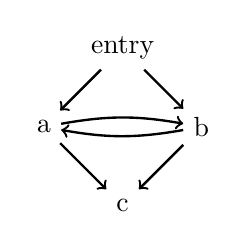
\begin{tikzpicture}[->, line width=0.3mm]
\node(entry) at (2,3) {entry};
\node(a) at (1,2) {a};
\node(b) at (3,2) {b};
\node(c) at (2,1) {c};
\path
  (entry) edge (a)
  (entry) edge (b)
  (a) edge [bend left=10] (b)
  (b) edge [bend left=10] (a)
  (a) edge (c)
  (b) edge (c);
\end{tikzpicture}
\end{column}
\begin{column}{0.5\textwidth}
\center
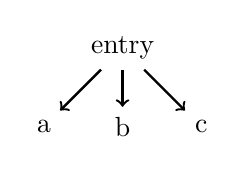
\begin{tikzpicture}[->, line width=0.3mm]
\node(entry) at (2,3) {entry};
\node(a) at (1,2) {a};
\node(b) at (2,2) {b};
\node(c) at (3,2) {c};
\path
(entry) edge (a)
(entry) edge (b)
(entry) edge (c);
\end{tikzpicture}
\end{column}
\end{columns}
\end{frame}

\begin{frame}[fragile]{Limitation of Dominator Trees}
\begin{columns}
\begin{column}{0.35\textwidth}
\begin{lstlisting}
define f(x){
  entry:
    cond = and x, 1
    br cond, @a@, &b&
  a: 
    y = mul 4, x
    call g()
    br cond, @b@, &c&
  b:
    z = add x, x
    call h()
    br cond, @c@, &a&
  c: 
    r = add y, z
    ret r
}
\end{lstlisting}
\end{column}
\begin{column}{0.3\textwidth}
\center
\textbf{\large{CFG}}\\
\vspace{0.5cm}
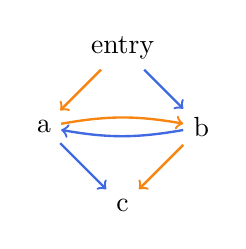
\begin{tikzpicture}[->, line width=0.3mm]
\node(entry) at (2,3) {entry};
\node(a) at (1,2) {a};
\node(b) at (3,2) {b};
\node(c) at (2,1) {c};
\path
  (entry) edge [color=BurntOrange] (a)
  (entry) edge [color=RoyalBlue] (b)
  (a) edge [color=BurntOrange,bend left=10] (b)
  (b) edge [color=RoyalBlue,bend left=10] (a)
  (a) edge [color=RoyalBlue] (c)
  (b) edge [color=BurntOrange] (c);
\end{tikzpicture}
\end{column}
\begin{column}{0.3\textwidth}
\center
\textbf{\large{DomTree}}\\
\vspace{0.5cm}
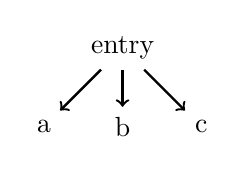
\begin{tikzpicture}[->, line width=0.3mm]
\node(entry) at (2,3) {entry};
\node(a) at (1,2) {a};
\node(b) at (2,2) {b};
\node(c) at (3,2) {c};
\path
(entry) edge (a)
(entry) edge (b)
(entry) edge (c);
\end{tikzpicture}
\end{column}
\end{columns}
\end{frame}

\begin{frame}[fragile]{Dominator DAG}
\begin{columns}
\begin{column}{0.35\textwidth}
\begin{lstlisting}
define f(x){
  entry:
    cond = and x, 1
    br cond, @a@, &b&
  a: 
    y = mul 4, x
    call g()
    br cond, @b@, &c&
  b:
    z = add x, x
    call h()
    br cond, @c@, &a&
  c: 
    r = add y, z
    ret r
}
\end{lstlisting}
\end{column}
\begin{column}{0.3\textwidth}
\center
\textbf{\large{CFG}}\\
\vspace{0.5cm}
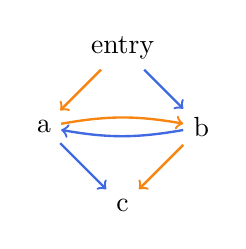
\begin{tikzpicture}[->, line width=0.3mm]
\node(entry) at (2,3) {entry};
\node(a) at (1,2) {a};
\node(b) at (3,2) {b};
\node(c) at (2,1) {c};
\path
  (entry) edge [color=BurntOrange] (a)
  (entry) edge [color=RoyalBlue] (b)
  (a) edge [color=BurntOrange,bend left=10] (b)
  (b) edge [color=RoyalBlue,bend left=10] (a)
  (a) edge [color=RoyalBlue] (c)
  (b) edge [color=BurntOrange] (c);
\end{tikzpicture}
\end{column}
\begin{column}{0.3\textwidth}
\center
\textbf{\large{DomDAG}}\\
\vspace{0.5cm}
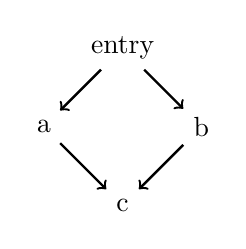
\begin{tikzpicture}[->, line width=0.3mm]
\node(entry) at (2,3) {entry};
\node(a) at (1,2) {a};
\node(b) at (3,2) {b};
\node(c) at (2,1) {c};
\path
(entry) edge (a)
(entry) edge (b)
(a) edge (c)
(b) edge (c);
\end{tikzpicture}
\end{column}
\end{columns}
\end{frame}

\begin{frame}{Formalization}
\center\textbf{Valid Paths}
$$\text{LLVM} \subseteq \text{\color{BurntOrange}{Conditional CFG}} \subseteq \text{\color{BurntOrange}{CFG}}$$

\vspace{0.5cm}

\center\textbf{Dominator Relation}
$$\text{\color{BurntOrange}{CFG}} \subseteq
\text{\color{BurntOrange}{Conditional CFG}} \subseteq \text{LLVM}$$
\end{frame}

\begin{frame}[fragile]{Concurrency}
\begin{columns}
\begin{column}{0.5\textwidth}
\center
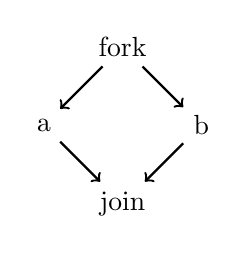
\begin{tikzpicture}[->, line width=0.3mm]
\node(entry) at (2,3) {fork};
\node(a) at (1,2) {a};
\node(b) at (3,2) {b};
\node(c) at (2,1) {join};
\path
(entry) edge (a)
(entry) edge (b)
(a) edge (c)
(b) edge (c);
\end{tikzpicture}
\end{column}
\end{columns}
\end{frame}

\begin{frame}[fragile]{Tapir}
\begin{columns}
\begin{column}{0.5\textwidth}
\center
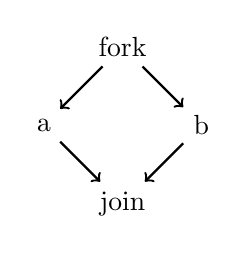
\begin{tikzpicture}[->, line width=0.3mm]
\node(entry) at (2,3) {fork};
\node(a) at (1,2) {a};
\node(b) at (3,2) {b};
\node(c) at (2,1) {join};
\path
(entry) edge (a)
(entry) edge (b)
(a) edge (c)
(b) edge (c);
\end{tikzpicture}
\end{column}
\begin{column}{0.5\textwidth}
\center
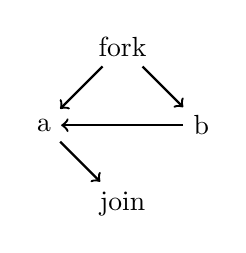
\begin{tikzpicture}[->, line width=0.3mm]
\node(entry) at (2,3) {fork};
\node(a) at (1,2) {a};
\node(b) at (3,2) {b};
\node(c) at (2,1) {join};
\path
  (entry) edge (a)
  (entry) edge (b)
  (b) edge (a)
  (a) edge (c); 
\end{tikzpicture}
\end{column}
\end{columns}
\end{frame}


\begin{frame}[fragile]{Concurrency}
\begin{columns}
\begin{column}{0.5\textwidth}
\center
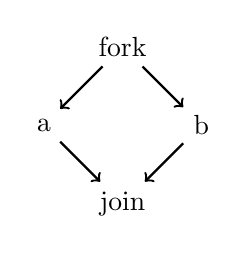
\begin{tikzpicture}[->, line width=0.3mm]
\node(entry) at (2,3) {fork};
\node(a) at (1,2) {a};
\node(b) at (3,2) {b};
\node(c) at (2,1) {join};
\path
(entry) edge (a)
(entry) edge (b)
(a) edge (c)
(b) edge (c);
\end{tikzpicture}
\end{column}
\begin{column}{0.5\textwidth}
\center
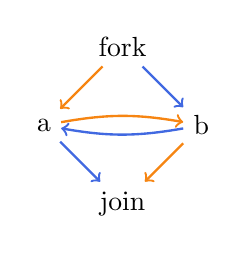
\begin{tikzpicture}[->, line width=0.3mm]
\node(entry) at (2,3) {fork};
\node(a) at (1,2) {a};
\node(b) at (3,2) {b};
\node(c) at (2,1) {join};
\path
  (entry) edge [color=BurntOrange] (a)
  (entry) edge [color=RoyalBlue] (b)
  (a) edge [color=BurntOrange,bend left=10] (b)
  (b) edge [color=RoyalBlue,bend left=10] (a)
  (a) edge [color=RoyalBlue] (c)
  (b) edge [color=BurntOrange] (c);
\end{tikzpicture}
\end{column}
\end{columns}
\end{frame}

\begin{frame}

\center
\huge{Questions?}

\end{frame}

\end{document}

